\documentclass[10pt]{beamer}

\usepackage{settings}


\title{From Latent to Deep Latent Variable Models}
\subtitle{A Study On Causal Effect Inference with CEVAE}
\date{June 17, 2025}
\author[longname]{Valeria De Stasio, Christian Faccio, Giovanni Lucarelli}
\titlegraphic{\hfill
\includegraphics[height=1.3cm]{images/logo100_orizzontale.pdf}}

% add graphics path
\graphicspath{{../assets},{./images}}

\begin{document}

\maketitle

% magari un frame iniziale in cui introduciamo il concetto di causalità?
\begin{frame}{Objective: estimating causal effects}
    Estimate how a medical treatment $T$ affects the health $Y$ of a \textit{random} patient.
  \begin{figure}
    \centering
    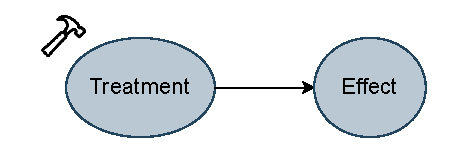
\includegraphics[width=0.7\textwidth]{images/no_confounders.pdf}
  \end{figure}

  \begin{equation*}
    P(Y=y|\text{do}(T=t))=P(Y=y|T=t)
  \end{equation*}
  \begin{equation*}
    \text{ITE} = \mathbb{E}[(Y|\text{do}(T=1)]-\mathbb{E}[(Y|\text{do}(T=0)]
  \end{equation*}
  
  This is usually the case in a \textbf{randomized controlled trial} (RCT), where the treatment is randomly assigned to the patients.

\end{frame}


% How to intervene on already observed data?
\begin{frame}{Confounder}
  In a observational study:
  \begin{itemize}
    \item \textbf{no} control over the treatment $T$ assignment\\
    $\rightarrow$ there may be a confounder $X$ (e.g. Income) that influences both variables
  \end{itemize}
  \begin{columns}
    \begin{column}{0.5\textwidth}
      \begin{equation*}
        P(Y|\text{do}(t))\ne P(Y|t)
      \end{equation*}
      \begin{equation*}
        P(Y|\text{do}(t),x) =P(Y|t,x)
      \end{equation*}
    \end{column}
    \begin{column}{0.5\textwidth}
      \begin{figure}
        \centering
        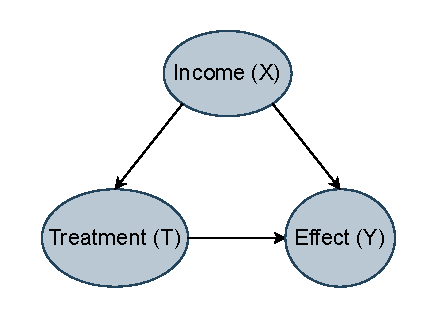
\includegraphics[width=\textwidth]{images/unconfoundness.pdf}
      \end{figure}
    \end{column}
  \end{columns}

  \centering{Here a linear rergession in principle can do the job!}
\end{frame}

\begin{frame}{Latent confounder}
But what if the confounder $Z$ (e.g. Wealth) is \textbf{not} observed and the observed $X$ is only a proxy of it?
    \begin{center}
  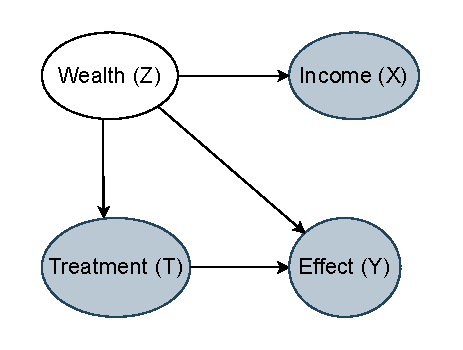
\includegraphics[width=0.5\textwidth]{images/latent_confounder.pdf}
\end{center}
  
\textbf{Idea:} estimate the latent variable and condition on it!
% \begin{itemize}
%     \item Latent Variable Model
%     \item Deep Latent Variable Model
% \end{itemize} 

 \end{frame}

 \begin{frame}{Vanilla Latent Variable Model}
     \begin{itemize}
         \item Assume parametric distributions
         \item Assume parametric relationships between variables
         \item Infer parameters using Stochastic Variational Inference (SVI)
     \end{itemize}

     \textbf{Problem:} to infer from new data point $x$ we need to train a new model at test time! 
 \end{frame}

  \begin{frame}{Deep Latent Variable Model: CEVAE}
     \begin{itemize}
         \item Assume parametric distributions
         \item Assume parametric relationships between variables through \alert{Neural Networks}
     \end{itemize}
    No need for test time training! \textbf{amortized inference}

 \end{frame}

\begin{frame}{Synthetic linear dataset}
    \begin{minipage}{0.48\textwidth}
      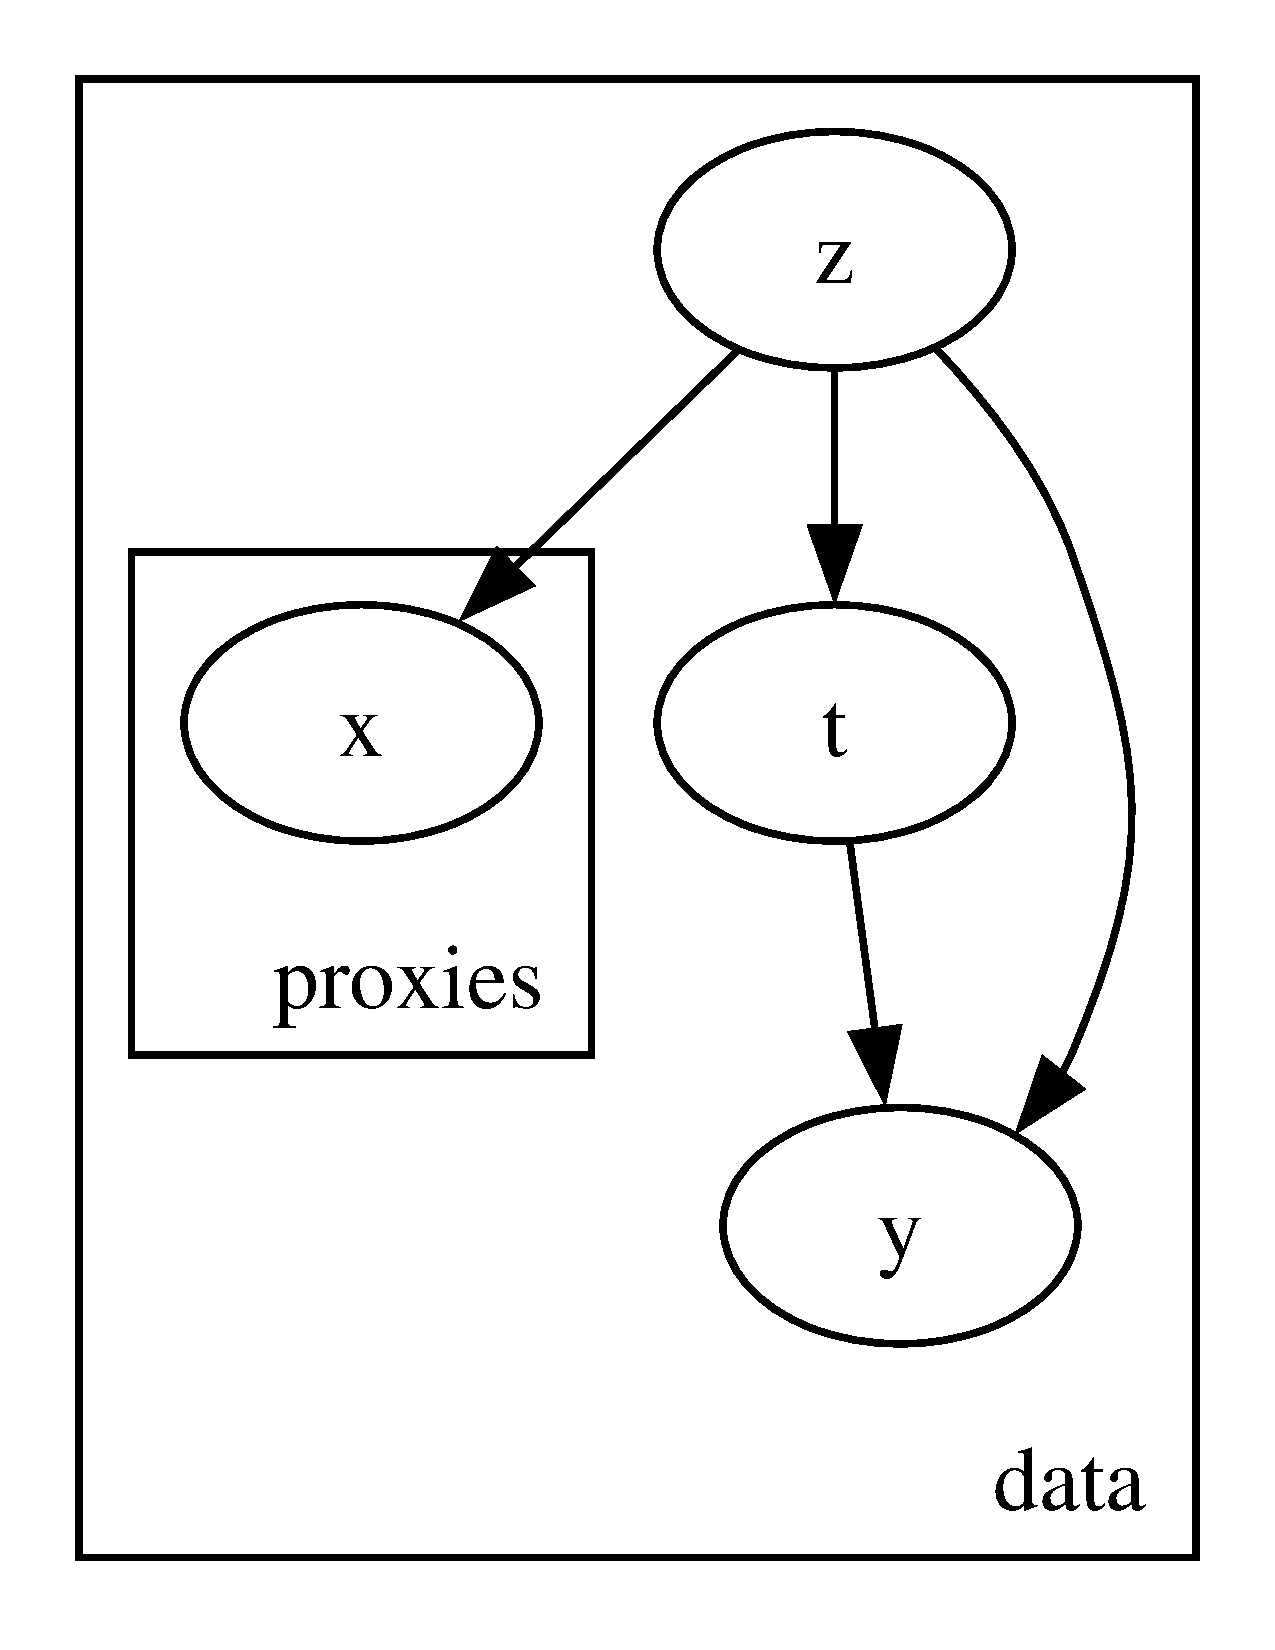
\includegraphics[width=0.9\textwidth]{images/pyro_model.pdf}
    \end{minipage}
    \begin{minipage}{0.48\textwidth}
        \begin{equation*}
        Z \sim \mathcal{N}(0,1)
        \end{equation*}
        \begin{equation*}
             a_j \sim \mathcal{U}(-10,10)
        \end{equation*}
        \begin{equation*}
        X_j \sim \mathcal{N}(a_j z,\sigma_X^2)\,    
        \end{equation*}
        \begin{equation*}
        T | Z \sim \text{Be}(\sigma(\beta z))    
        \end{equation*}
        \small{\begin{equation*}
        Y|T,Z \sim \mathcal{N}(z + t, \sigma_Y^2)            
        \end{equation*}}
      \end{minipage}
      \centering
      {\textbf{Remark:} ITE is constant for all  $x$!}
\end{frame}

\begin{frame}{Synthetic non linear dataset}
    \begin{minipage}{0.48\textwidth}
    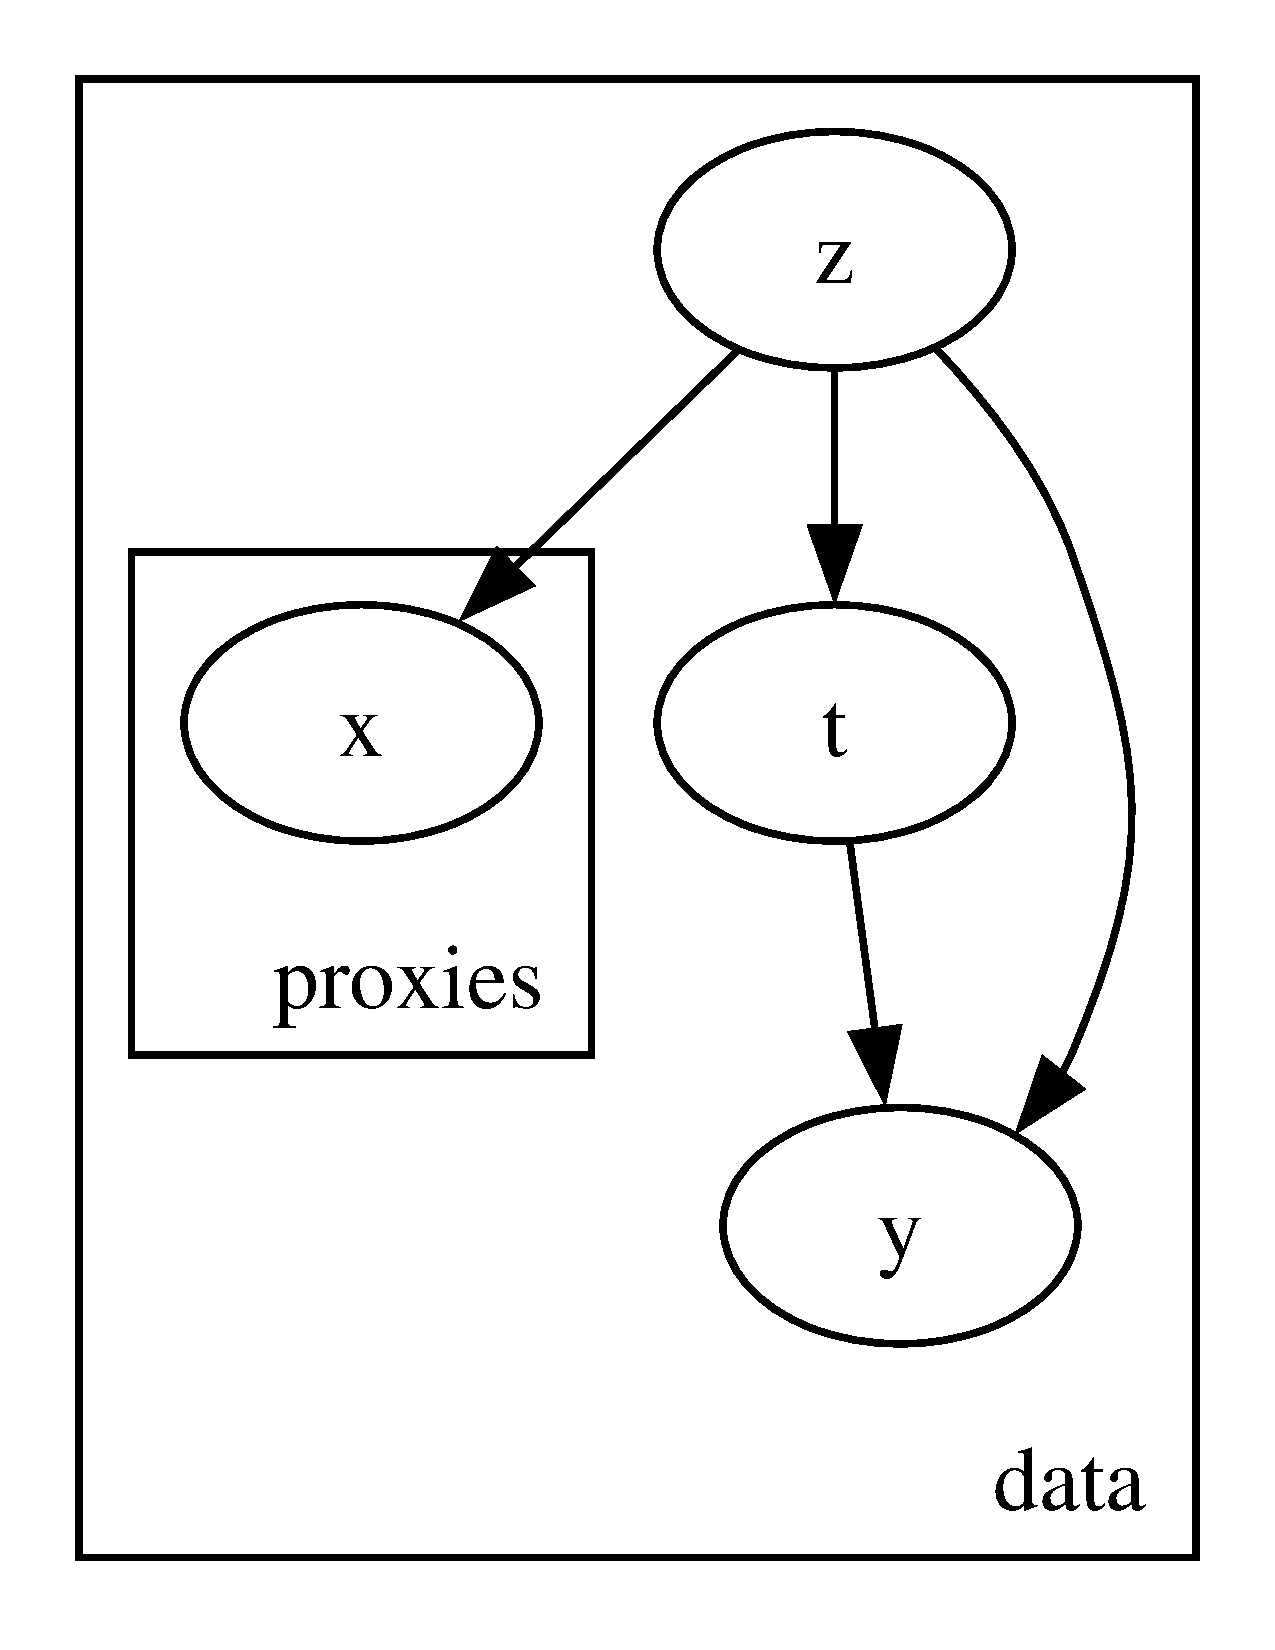
\includegraphics[width=0.9\textwidth]{images/pyro_model.pdf}
    \end{minipage}
    \begin{minipage}{0.48\textwidth}
    
        \begin{equation*}
        Z \sim \mathcal{N}(0,1)
        \end{equation*}
        \begin{equation*}
            a \sim \mathcal{U}(-10,10)^d
        \end{equation*}
        \begin{equation*}
        \Sigma=\sigma_X^2[(1-\rho) \mathbb{I}+\rho J]    
        \end{equation*}
        \begin{equation*}
        X_1,...,X_d \sim \mathcal{N}(a\tanh(z),\Sigma)     
        \end{equation*}
        \begin{equation*}
        T | Z \sim \text{Be}(\sigma(\beta z))    
        \end{equation*}
        \begin{equation*}
        Y|T,Z \sim \mathcal{N}\left(\text{NonLin}(z,t),\sigma_Y^2\right)           
        \end{equation*}
        \begin{equation*}
        \text{NonLin}(z,t) = \sin(z)+\frac12z+t\left(1+\frac12z\right)      
        \end{equation*}
    \end{minipage}
    
\end{frame}

\begin{frame}{Results (1/2): Linear Dataset}
    \begin{figure}[H]
      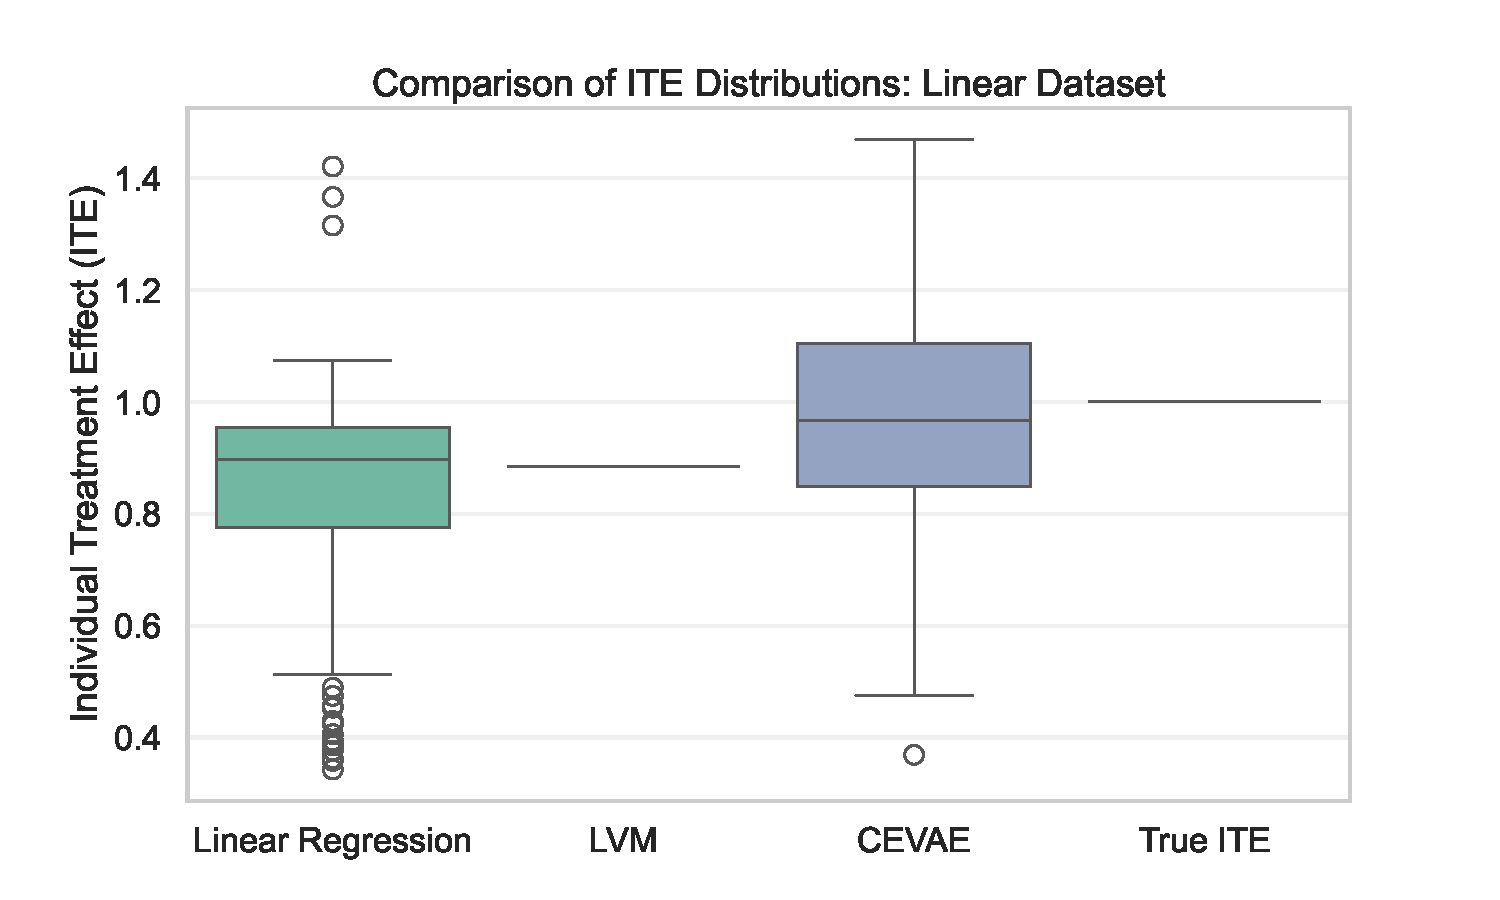
\includegraphics[width=\textwidth]{../src/results/boxplot_linear.pdf}
    \end{figure}
\end{frame}

\begin{frame}{Results (2/2): Non Linear Dataset}
    \begin{figure}[H]
      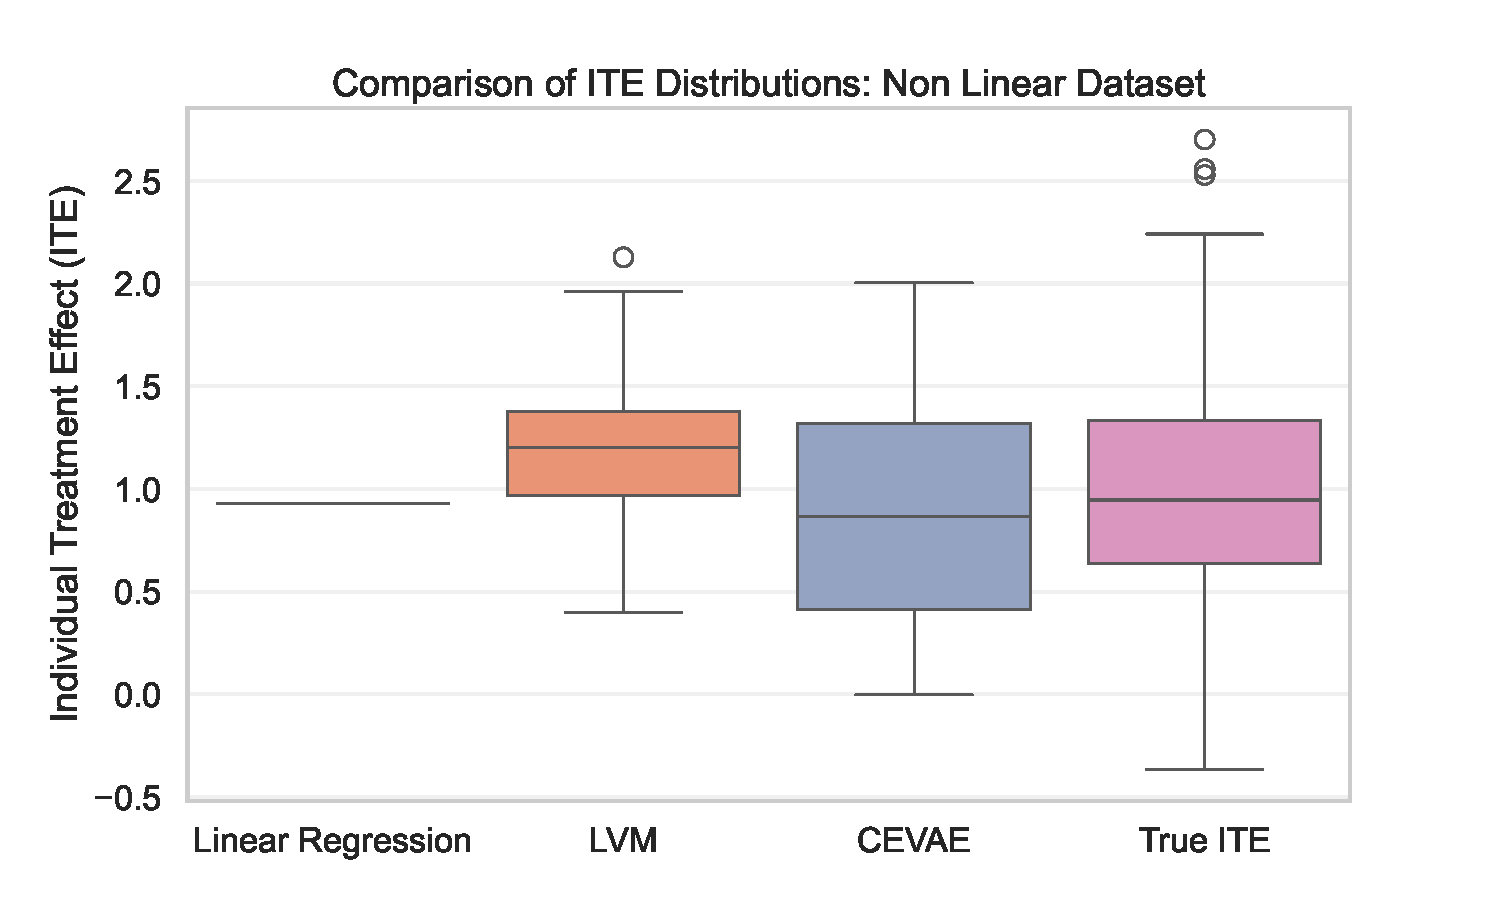
\includegraphics[width=\textwidth]{../src/results/boxplot_non_linear.pdf}
    \end{figure}
\end{frame}

\begin{frame}{Experiment 1: Increasing the sample size}
  \begin{figure}[H]
      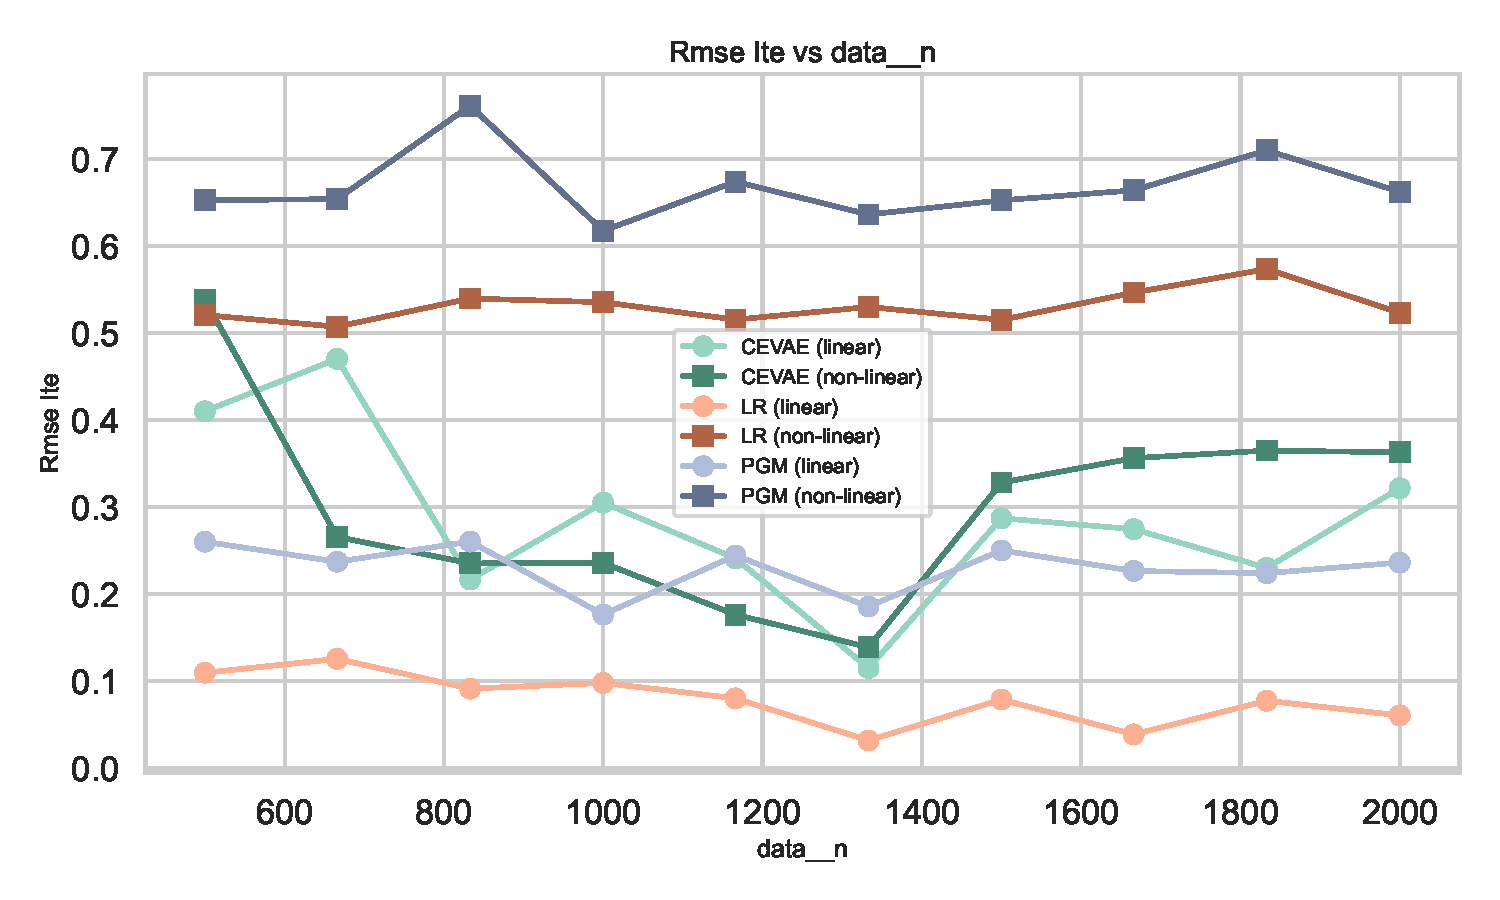
\includegraphics[width=\textwidth]{../src/results/MyRun_data__n--rmse_ite.pdf}
    \end{figure}
\end{frame}

\begin{frame}{Experiment 2: Increasing correlation among proxies}
  \begin{figure}[H]
      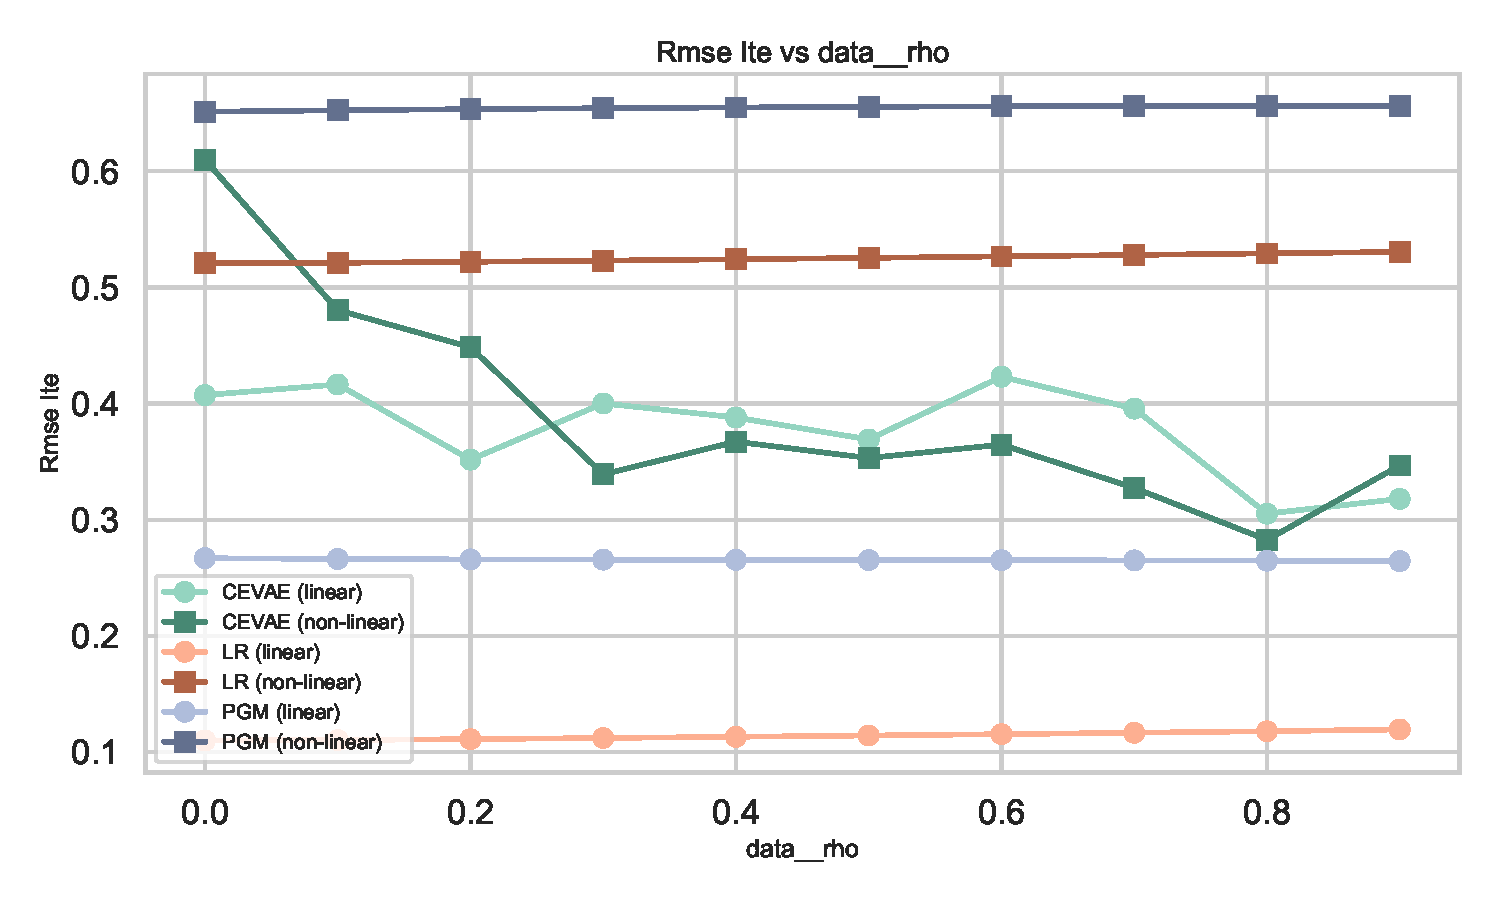
\includegraphics[width=\textwidth]{../src/results/MyRun_data__rho--rmse_ite.pdf}
    \end{figure}
\end{frame}

\begin{frame}{Experiment 3: Increasing decorrelation among proxies}
    \begin{figure}[H]
      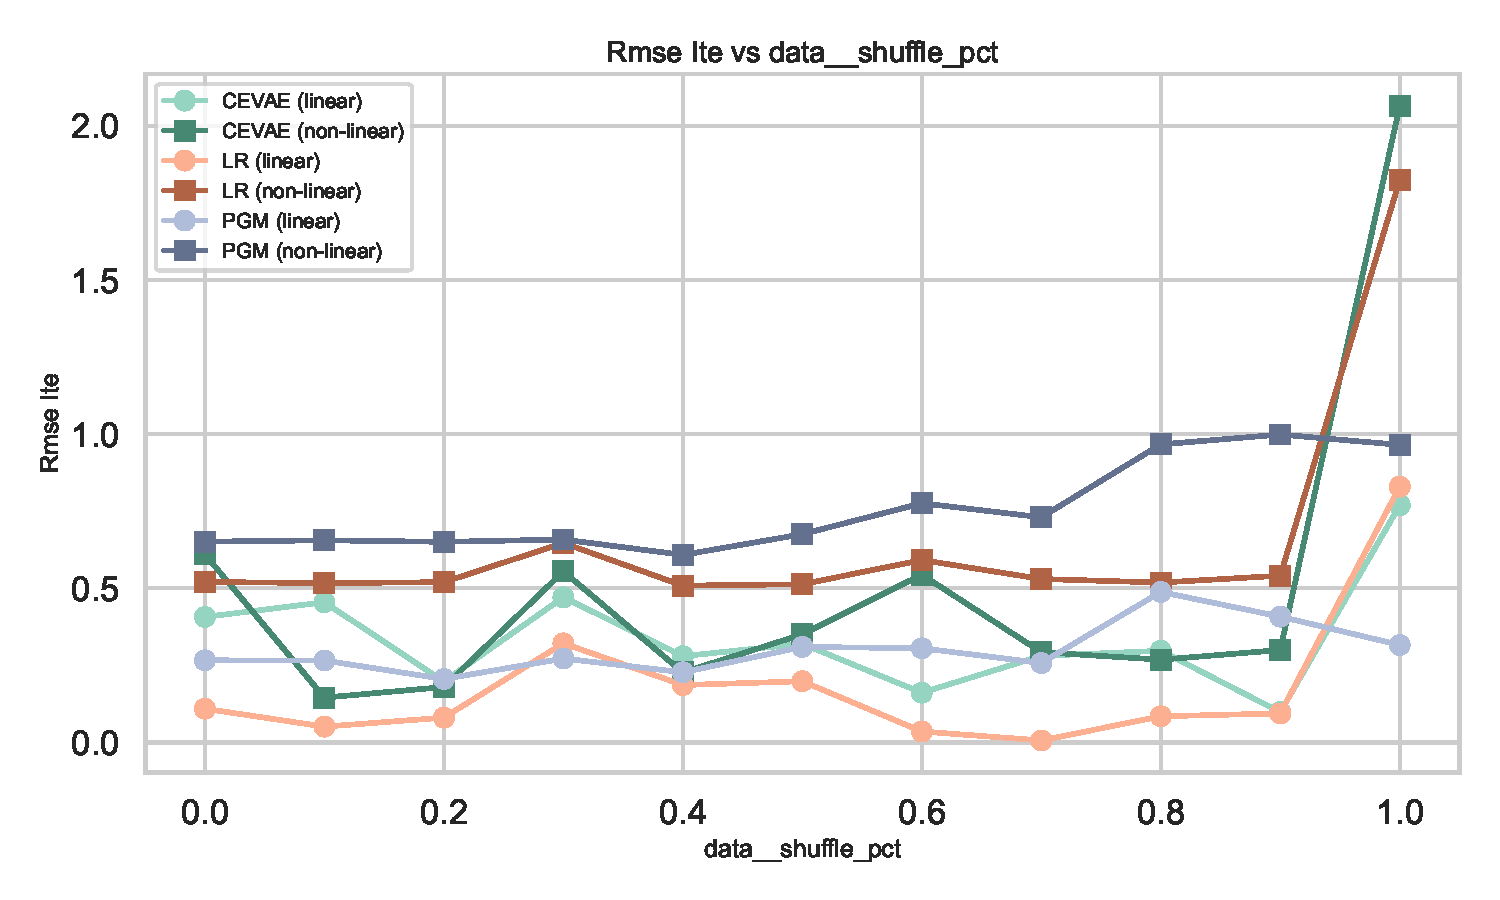
\includegraphics[width=\textwidth]{../src/results/MyRun_data__shuffle_pct--rmse_ite.pdf}
    \end{figure}
  \begin{figure}[H]
      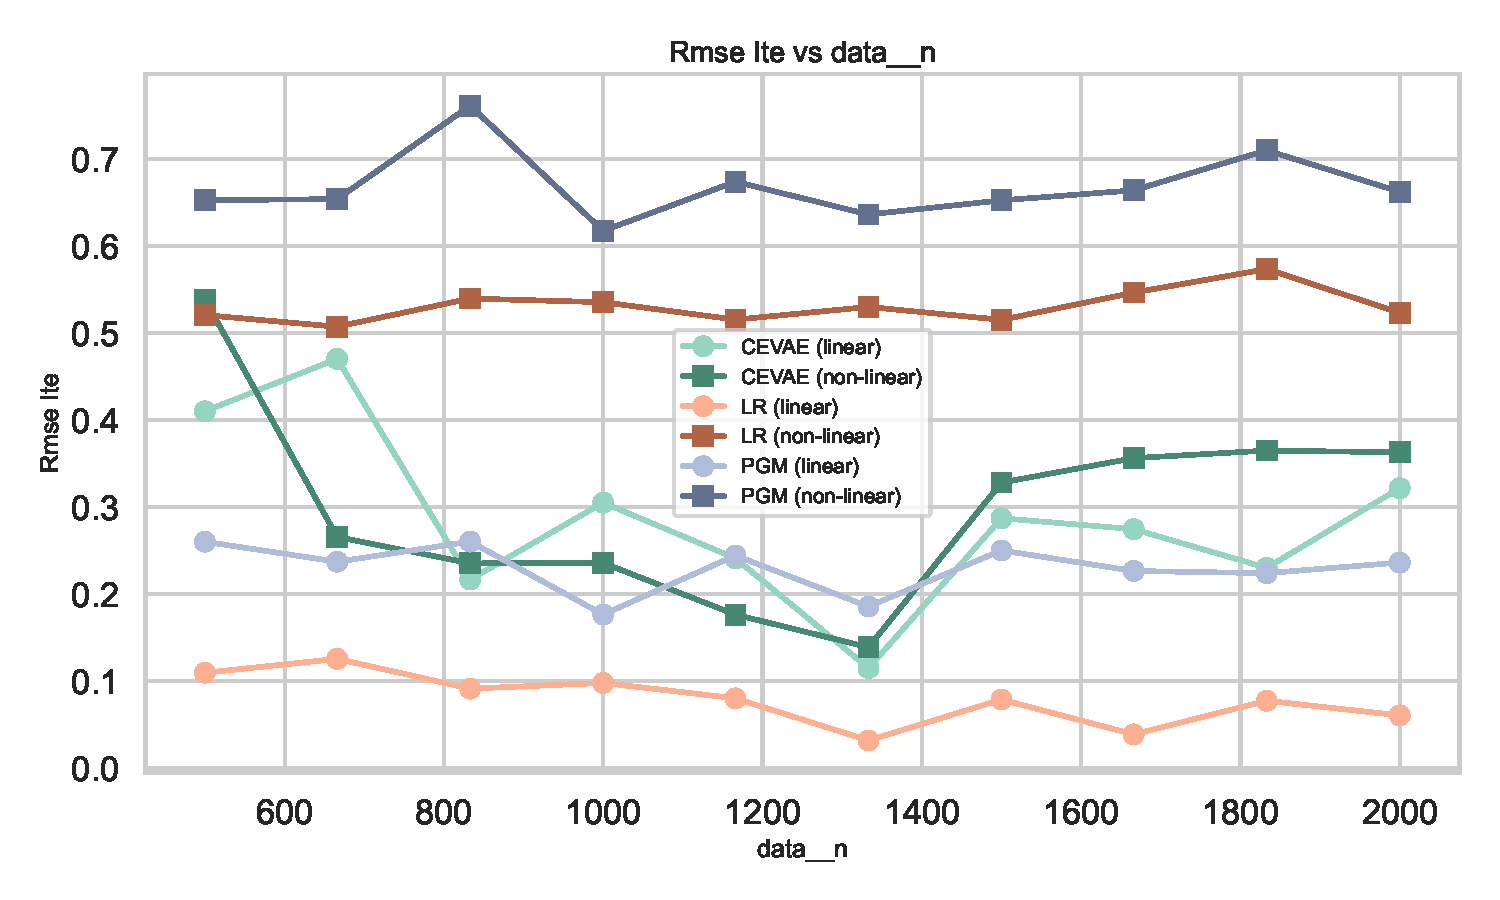
\includegraphics[width=\textwidth]{../src/results/MyRun_data__n--rmse_ite.pdf}
    \end{figure}
\end{frame}

\begin{frame}{Experiment 4: Increasing latent dimension}
    \begin{figure}[H]
      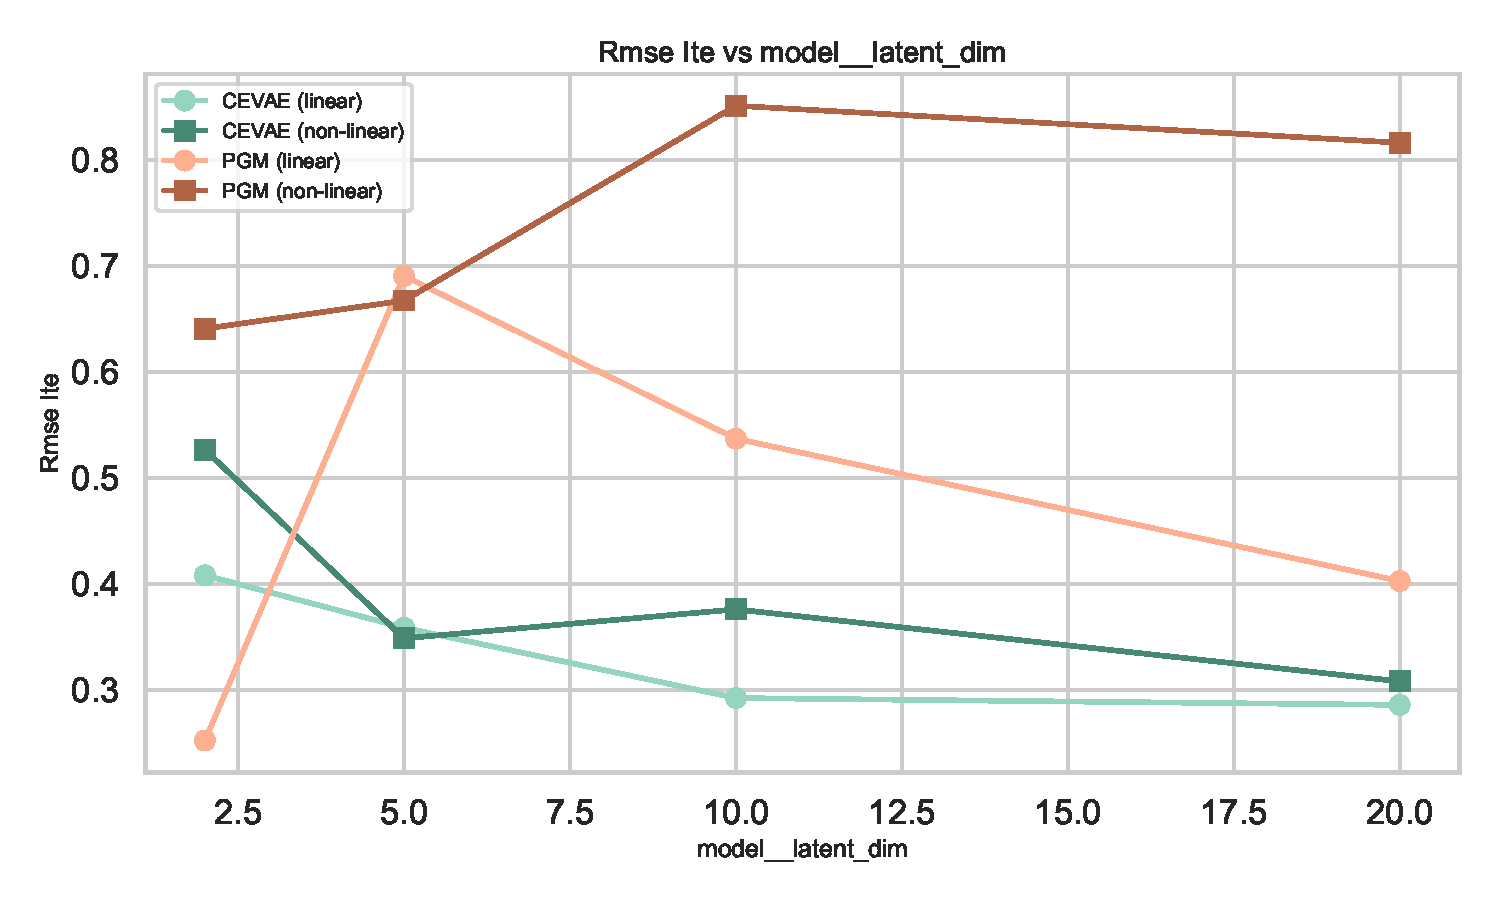
\includegraphics[width=\textwidth]{../src/results/MyRun_model__latent_dim--rmse_ite.pdf}
    \end{figure}
\end{frame}

\begin{frame}{Experiment 5: latent distribution misspecified}
    \begin{figure}[H]
      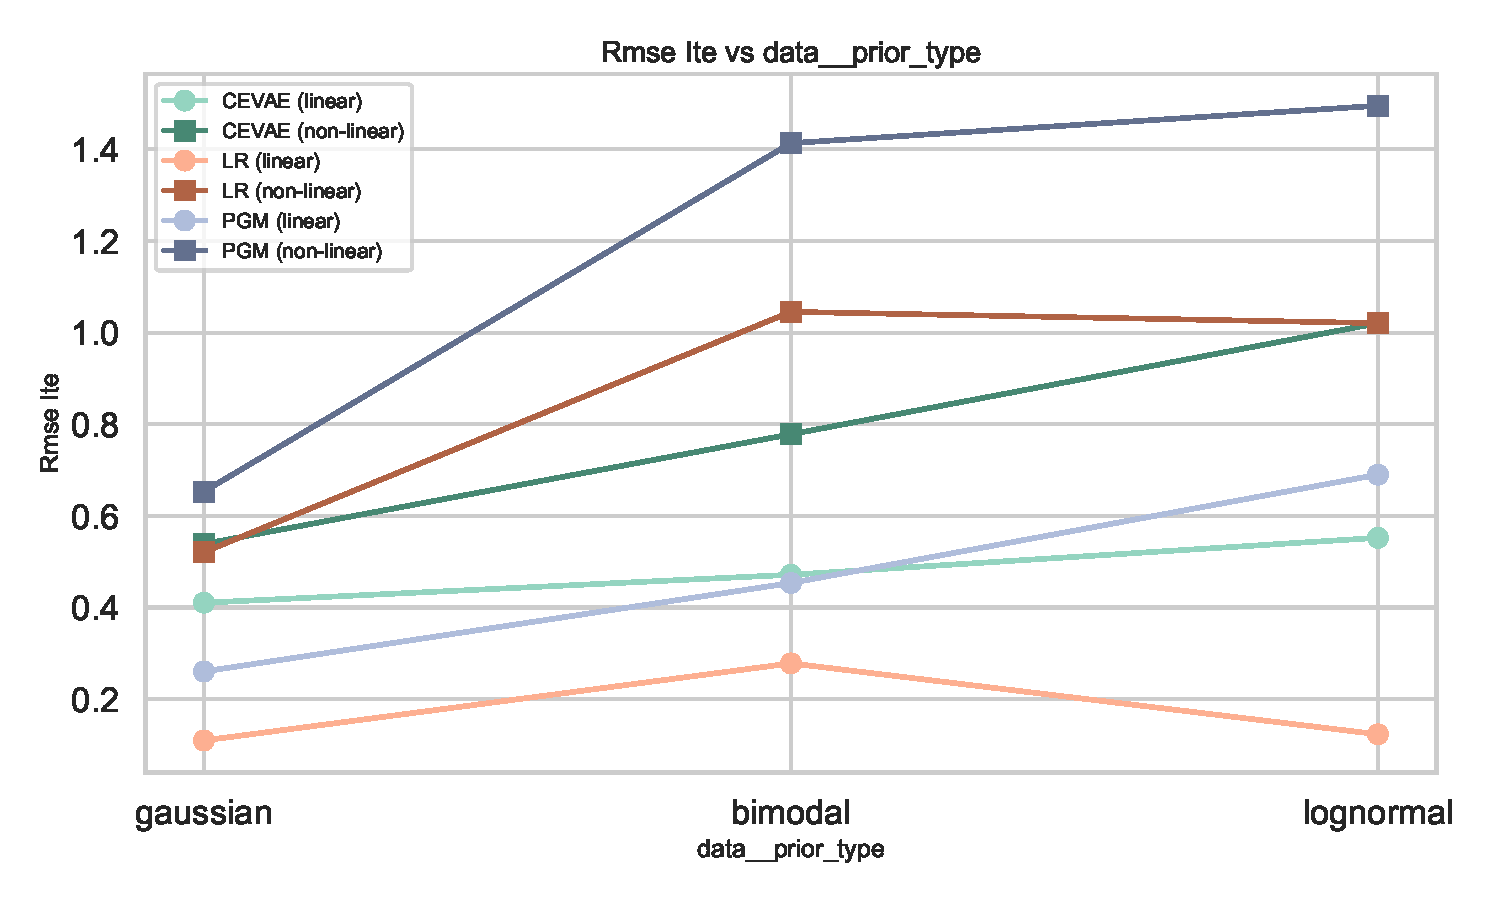
\includegraphics[width=\textwidth]{../src/results/MyRun_data__prior_type--rmse_ite.pdf}
    \end{figure}
\end{frame}

\begin{frame}{Experiment 6: Increasing the number of proxies}
    \begin{figure}[H]
      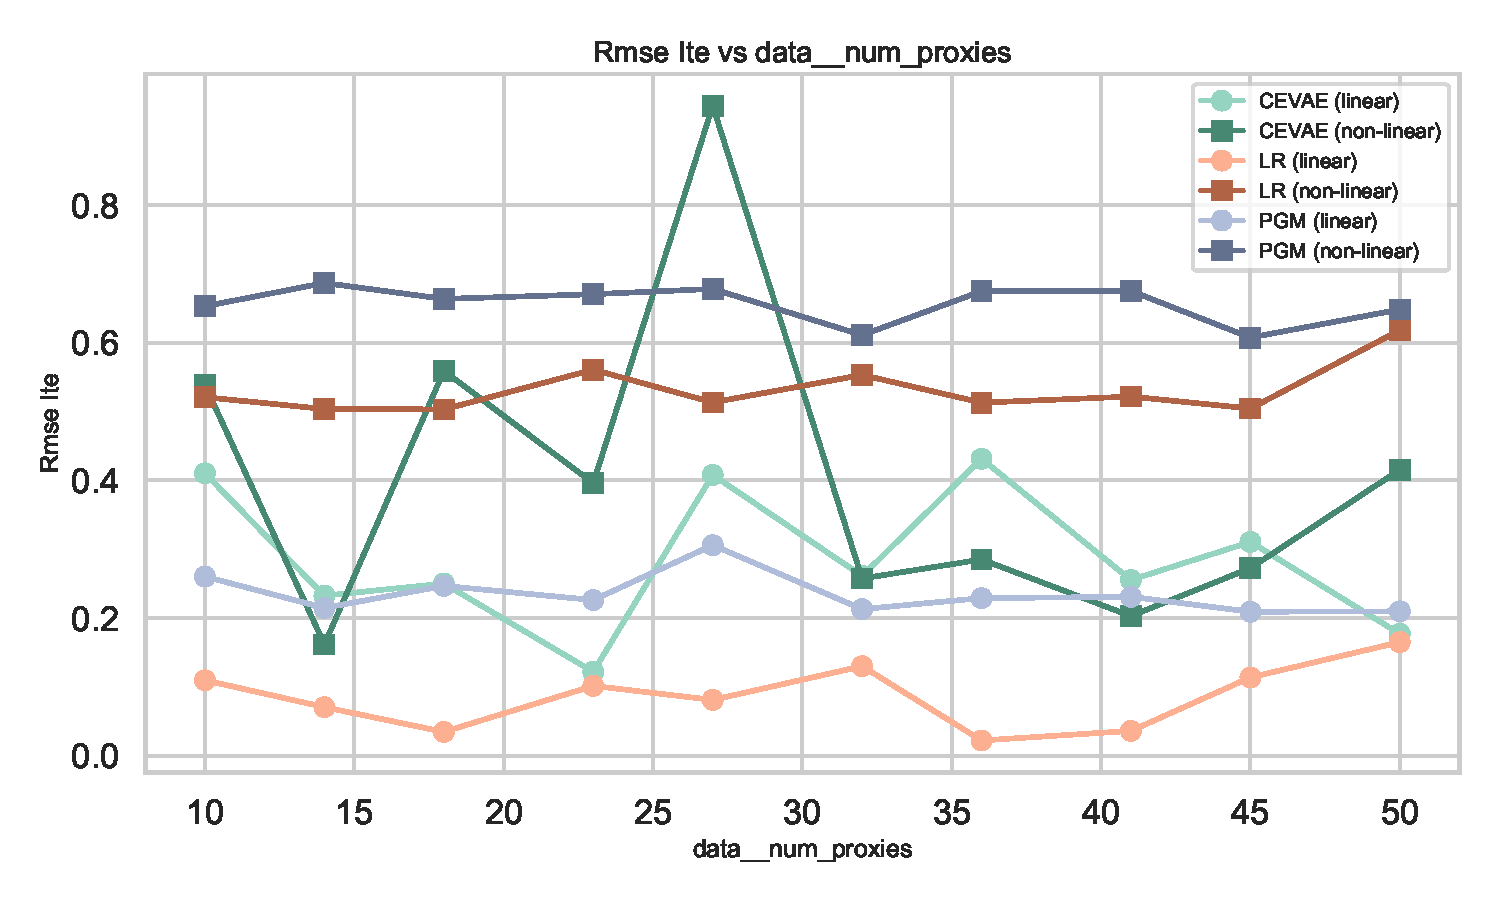
\includegraphics[width=\textwidth]{../src/results/MyRun_data__num_proxies--rmse_ite.pdf}
    \end{figure}
\end{frame}

\begin{frame}{Conclusions}

\end{frame}

{\setbeamercolor{palette primary}{fg=white, bg=bluscuro}
\begin{frame}[standout]
\thispagestyle{empty}
  {\LARGE Thank You!}
\end{frame}
}



\end{document}